\documentclass[thnuscript,10pt,number,sort&compress]{elsarticle}


%%%%%%%%%%%%%%%%%%%%%%%%%%%%%%%%%%%%%%%%%%%%%%%%%%%%%%%%%%%%%%%%%%%%%%%%%%%%%%%%%%%%%%%%%%%%%%%%%%%%%%%%%
\usepackage{csquotes,xpatch}% recommended

%%%%%%%%%%%%%%%%%%%%%%%%%%%%%%%%%%%%%%%%%%%%%%%%%%%%%%%%%%%%%%%%%%%%%%%%%%%%%%%%%%%%%%%%%%%%%%%%%%%%%%%%%
\usepackage{graphicx}
\usepackage{epstopdf} 
%%%%%%%%%%%%%%%%%%%%%%%%%%%%%%%%%%%%%%%%%%%%%%%%%%%%%%%%%%%%%%%%%%%%%%%%%%%%%%%%%%%%%%%%%%%%%%%%%%%%%%%%%
\usepackage{calrsfs}
\usepackage{physics}
\usepackage{mathtools}  
\usepackage{amsmath}
\usepackage{amssymb}
\usepackage{tabulary}
\usepackage{booktabs}

%%%%%%%%%%%%%%%%%%%%%%%%%%%%%%%%%%%%%%%%%%%%%%%%%%%%%%%%%%%%%%%%%%%%%%%%%%%%%%%%%%%%%%%%%%%%%%%%%%%%%%%%%

\linespread{1.2}
\usepackage{geometry}
\geometry{
	a4paper,
	total={166mm,251mm},
	left=22mm,
	top=22mm,
	headsep=.5in
}
\raggedbottom
%%%%%%%%%%%%%%%%%%%%%%%%%%%%%%%%%%%%%%%%%%%%%%%%%%%%%%%%%%%%%%%%%%%%%%%%%%%%%%%%%%%%%%%%%%%%%%%%%%%%%%%%%
\usepackage{blindtext}
\usepackage{ragged2e}
\usepackage{float}

\usepackage{epstopdf}
\usepackage{empheq} 

\usepackage{array}

%%%%%%%%%%%%%%%%%%%%%%%%%%%%%%%%%%%%%%%%%%%%%%%%%%%%%%%%%%%%%%%%%%%%%%%%%%%%%%%%%%%%%%%%%%%%%%%%%%%%%%%%%
\usepackage{graphics}
\graphicspath{ {figures/} }
\renewcommand{\listfigurename}{List of figures}

\usepackage[labelfont=bf,justification=justified,singlelinecheck=false]{caption}
\captionsetup[figure]{name=Fig. ,labelsep=period}
\captionsetup[table]{labelsep=newline,font=footnotesize}
\captionsetup[figure]{labelfont={bf},labelformat={default},labelsep=period,name={Fig.},font=footnotesize}
%%%%%%%%%%%%%%%%%%%%%%%%%%%%%%%%%%%%%%%%%%%%%%%%%%%%%%%%%%%%%%%%%%%%%%%%%%%%%%%%%%%%%%%%%%%%%%%%%%%%%%%%%
\usepackage{array}
\usepackage{longtable}
\usepackage[dvipsnames]{xcolor}

\usepackage{comment}

\usepackage[shortlabels]{enumitem}

\usepackage{wrapfig}
%%%%%%%%%%%%%%%%%%%%%%%%%%%%%%%%%%%%%%%%%%%%%%%%%%%%%%%%%%%%%%%%%%%%%%%%%%%%%%%%%%%%%%%%%%%%%%%%%%%%%%%%%

% \newcommand{\hsp}{\hspace{5pt}}

%%%%%%%%%%%%%%%%%%%%%%%%%%%%%%%%%%%%%%%%%%%%%%%%%%%%%%%%%%%%%%%%%%%%%%%%%%%%%%%%%%%%%%%%%%%%%%%%%%%%%%%%%
\usepackage{subcaption}
\usepackage{bbm}
\usepackage{tabularx}

\usepackage{indentfirst}

%%%%%%%%%%%%%%%%%%%%%%%%%%%%%%%%%%%%%%%%%%%%%%%%%%%%%%%%%%%%%%%%%%%%%%%%%%%%%%%%%%%%%%%%%%%%%%%%%%%%%%%%

\usepackage{subcaption}

\usepackage[english]{babel}
\usepackage{blindtext}
\usepackage{amsmath,amsthm}
\usepackage{rotating}
% \usepackage[subfigure]{tocloft}

\DeclareMathOperator*{\argmin}{arg\,min}

\DeclareMathAlphabet{\pazocal}{OMS}{zplm}{m}{n}
\newcommand{\cH}{\pazocal{H}}
\newcommand{\cN}{\pazocal{N}}
\newcommand{\cP}{\pazocal{P}}
\newcommand{\cD}{\pazocal{D}}
\newcommand{\cO}{\pazocal{O}}
\newcommand{\cL}{\pazocal{L}}

\usepackage[ruled,vlined]{algorithm2e}
\SetKwComment{Comment}{$\triangleright$\ }{}

\usepackage{geometry}
\usepackage{marginnote}

\usepackage{dsfont}
\usepackage{diagbox}

\usepackage{multirow} 
\usepackage{multicol}

\usepackage[titletoc]{appendix}

\usepackage{pdflscape}
\usepackage{fancyhdr} 

\fancypagestyle{mylandscape}{
\fancyhf{} %Clears the header/footer
\fancyfoot{% Footer
\makebox[\textwidth][r]{% Right
  \rlap{\hspace{.75cm}% Push out of margin by \footskip
    \smash{% Remove vertical height
      \raisebox{4.87in}{% Raise vertically
        \rotatebox{90}{\thepage}}}}}}% Rotate counter-clockwise
\renewcommand{\headrulewidth}{0pt}% No header rule
\renewcommand{\footrulewidth}{0pt}% No footer rule
}

%%%%%%%%%%%%%%%%%%%%%%%%%%%%%%%%%%%%%%%%%%%%%%%%%%%%%%%%%%%%%%%%%%%%%%%%%%%%%%%%%%%%%%%%%%%%%%%%%%%%%%%%%
\usepackage[hyperfootnotes=false]{hyperref}

\definecolor{mycolor}{RGB}{207,42,40}
\hypersetup{
	colorlinks
}

\AtBeginDocument{\hypersetup{citecolor=mycolor, linkcolor = mycolor}}
%%%%%%%%%%%%%%%%%%%%%%%%%%%%%%%%%%%%%%%%%%%%%%%%%%%%%%%%%%%%%%%%%%%%%%%%%%%%%%%%%%%%%%%%%%%%%%%%%%%%%%%%%
\setcounter{tocdepth}{2}

\usepackage{etoc}
\def\TOCverysmallvskip {0pt plus .2pt}

% \usepackage[T1]{fontenc}
%%%%%%%%%%%%%%%%%%%%%%%%%%%%%%%%%%%%%%%%%%%%%%%%%%%%%%%%%%%%%%%%%%%%%%%%%%%%%%%%%%%%%%%%%%%%%%%%%%%%%%%%%
\makeatletter
\def\ps@pprintTitle{%
  \let\@oddhead\@empty
  \let\@evenhead\@empty
  \let\@oddfoot\@empty
  \let\@evenfoot\@oddfoot
}
\makeatother
%%%%%%%%%%%%%%%%%%%%%%%%%%%%%%%%%%%%%%%%%%%%%%%%%%%%%%%%%%%%%%%%%%%%%%%%%%%%%%%%%%%%%%%%%%%%%%%%%%%%%%%%%
\interfootnotelinepenalty=10000


\begin{document}
	
		\begin{frontmatter}
		
		\title{Title}
		
		\author[address1]{First~Author\corref{email}\fnref{comment}}
		\ead{email address}
		
		\author[address2]{Second~Author\fnref{comment}}
		
		\address[address1]{Address 1}
		\address[address2]{Address 2}
		
		\fntext[comment]{Comment.}
		\cortext[email]{Corresponding Author}
%		
%		\cortext[email]{Corresponding Author}\/ead{email address}
		
		\begin{abstract}
			Abstract. 					
		\end{abstract}
		
		\begin{keyword}
			keywords
		\end{keyword}
		
	\end{frontmatter}

	
	

	
	{\footnotesize
		\setlength{\parskip}{0.1em}
		\linespread{0.1}
		\tableofcontents
		}
	
	\section{Section}\label{sec:label}
	
	Text. Example citation \cite{abdar2021review}.
	
	\begin{figure}[!ht]
		\centering
		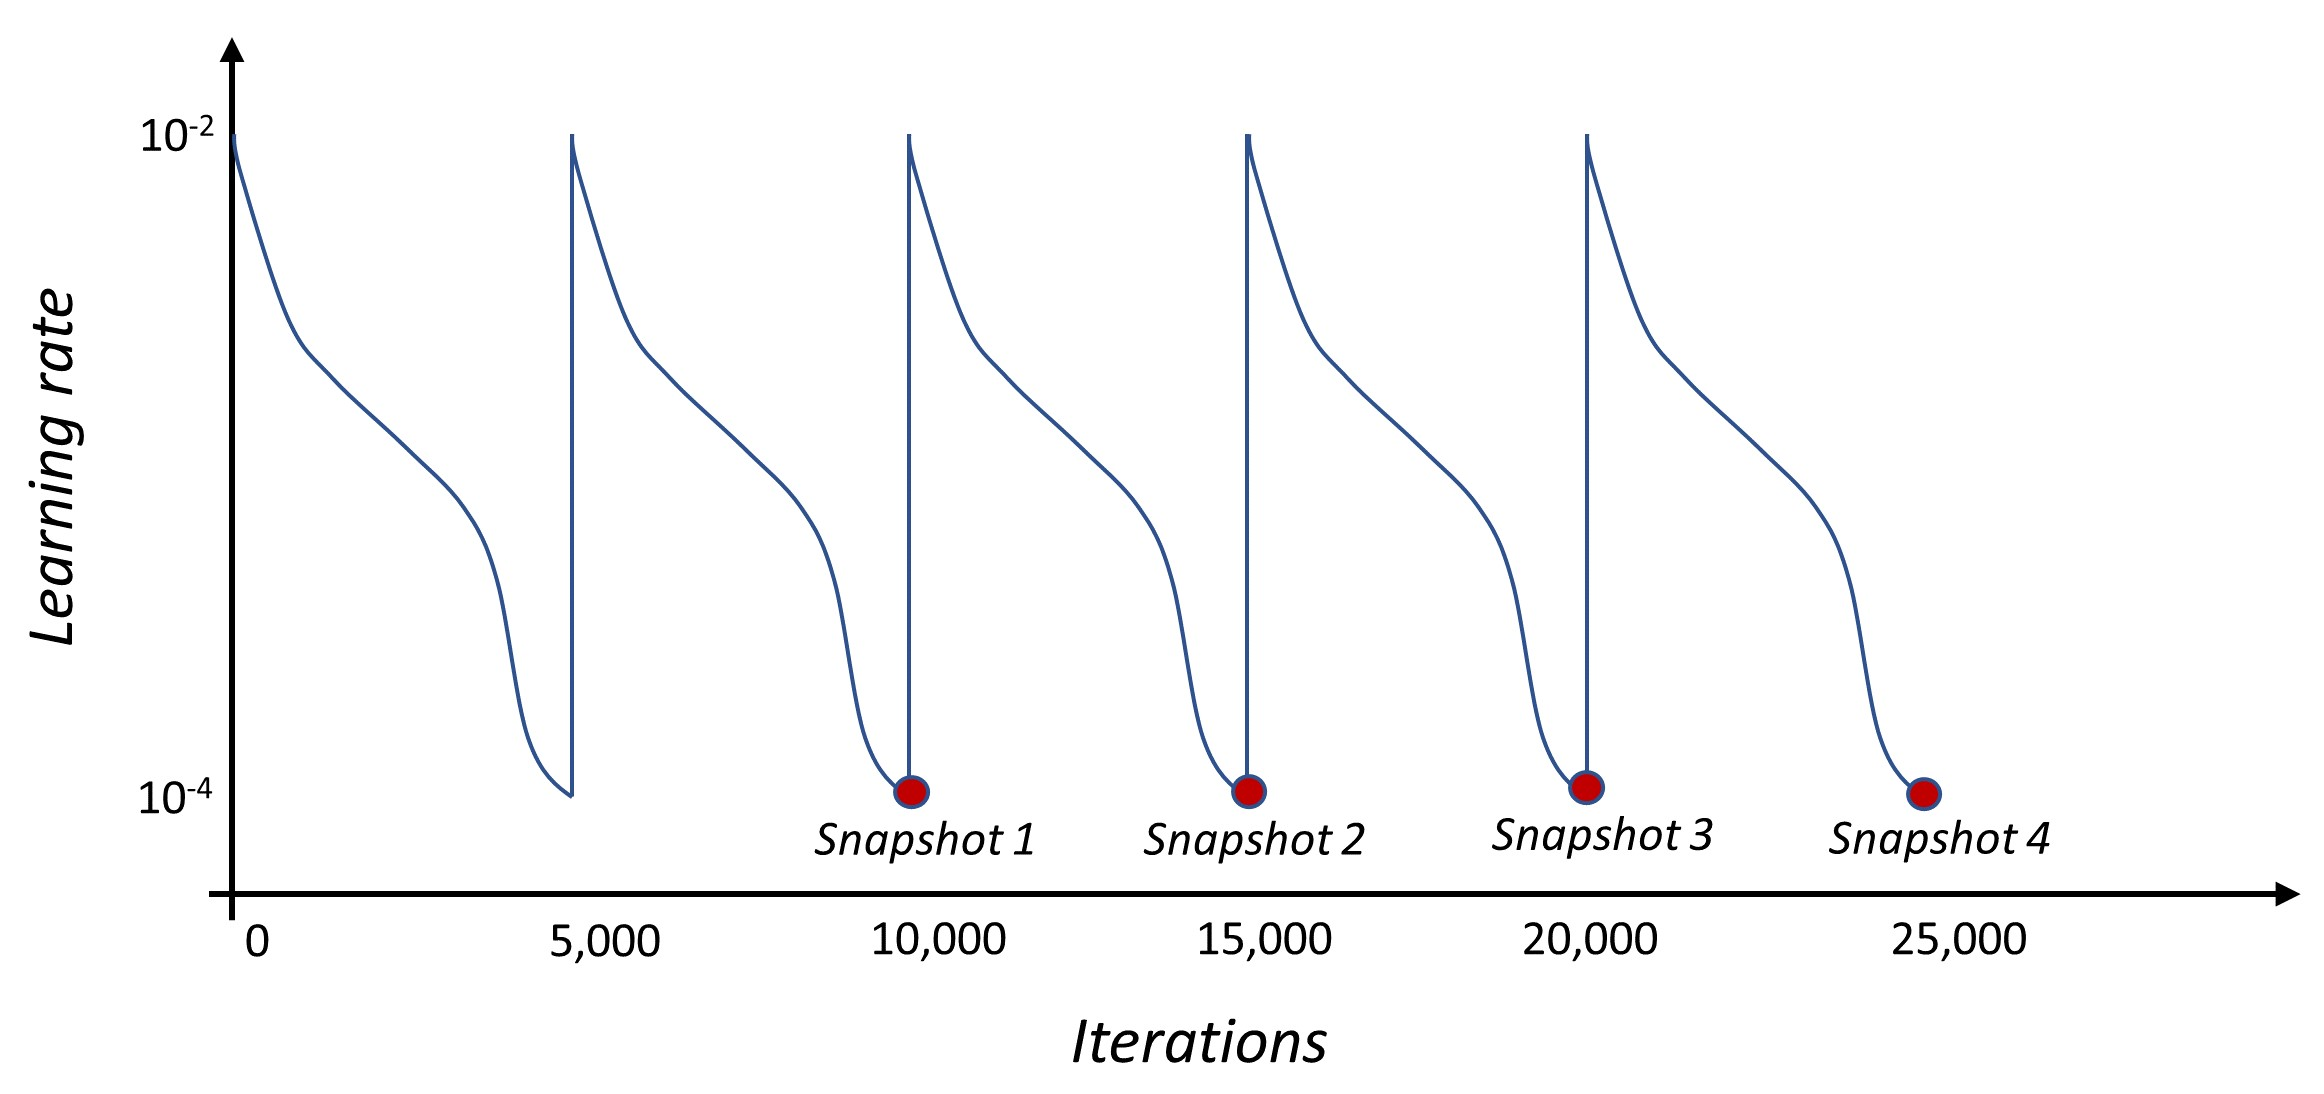
\includegraphics[width=.6\linewidth]{./figs/fig.jpg}
		\caption{Caption.
		}
		\label{fig:label}
	\end{figure} 

	\begin{equation}\label{eq:label}
		\hat{\theta} =  \underset{\theta}{\mathrm{argmin}}~\pazocal{L}(\theta) \text{, where } 
		\pazocal{L}(\theta) = \frac{1}{NN_u}\sum_{i=1}^{N}\sum_{j=1}^{N_u}
		||u_{\theta}(x_j^{(i)}; \xi_i) - u_j^{(i)}||_2^2    
	\end{equation}

	\begin{equation}\label{eq:label}
		Var(u|x, \cD) \approx \bar{\sigma}^2(x) =  \underbrace{\Sigma_{u}^2}_{\bar{\sigma}_a^2(x)}  + \underbrace{\frac{1}{M}\sum_{j=1}^M(u_{\hat{\theta}_j}(x)-\bar{\mu}(x))^2}_{\bar{\sigma}_e^2(x)}
	\end{equation} 
	
	\begin{subequations}\label{eq:label}
		\begin{align}
			\pazocal{F}_{\lambda, \xi}[u(x; \xi)] &= f(x; \xi) \text{, } x \in  \Omega\text{, } \xi \in \Xi, 
			\label{eq:label:a}\\
			\pazocal{B}_{\lambda, \xi}[u(x; \xi)] & = b(x; \xi) \text{, } x \in \Gamma, 
			\label{eq:label:b}
		\end{align}
	\end{subequations}
	
	\begin{equation}\label{eq:label}
		u(x) = \left\{
		\begin{aligned}
			&\frac{1}{2}[\sin^3(2 \pi x) - 1], ~ -1 \le x < 0, \\
			&\frac{1}{2}[\sin^3(3 \pi x) + 1], ~ 0 \le x \le 1.
		\end{aligned}
		\right.
	\end{equation}

	\begin{equation}
		\begin{aligned}\label{eq:label}
			p(\cD_f|\theta) & = \prod_{i=1}^{N_f}p(f_i|x_i, \theta) \text{; } & p(\cD_b|\theta) & = \prod_{i=1}^{N_b}p(b_i|x_i, \theta);\\
			p(\cD_u|\theta) & = \prod_{i=1}^{N_u}p(u_i|x_i, \theta) \text{; } & p(\cD_{\lambda}|\theta) & = \prod_{i=1}^{N_{\lambda}}p(\lambda_i|x_i, \theta)
		\end{aligned}
	\end{equation}

	\begin{table}[!ht] %[H]
		\centering
		\footnotesize
		\begin{tabular}{c|ccccccccc}
			\toprule
			Metric ($\times 10^2$)
			& GP & HMC & LD & MFVI & MCD & LA & DEns & SEns & SWAG \\
			\midrule
			RL2E ($\downarrow$) & 22.1 & 22.9 & 23.5 & 29.2 & \textbf{21.9} & 23.1 & 23.1 & 22.1 & 26.2 \\ 
			MPL ($\uparrow$) & 228.3 & 225.8 & 103.3 & 121.6 & 237.8 & 209.5 & 235.0 & \textbf{241.6} & 109.0 \\ 
			RMSCE ($\downarrow$) & \textbf{6.9} & 7.2 & 15.5 & 8.8 & 8.6 & 7.1 & 8.3 & 7.2 & 13.6 \\ 
			\midrule
			Cal RMSCE ($\downarrow$) & 6.8 & 6.7 & 6.4 & \textbf{3.8} & 8.0 & 6.5 & 6.5 & 6.9 & 5.7 \\ 
			PIW ($\downarrow$) & 45.8 & 45.2 & 142.0 & 116.2 & 42.5 & 51.9 & \textbf{40.5} & 41.9 & 132.0 \\ 
			SDCV ($\uparrow$) & 3.3 & 4.6 & 2.8 & \textbf{38.2} & 4.6 & 29.6 & 6.0 & 6.3 & 8.8 \\ 
			\bottomrule
		\end{tabular}
		\caption{
			Caption.
		}
		\label{tab:label}
	\end{table}
	
	\begin{figure}[!ht]
		\centering
		\subcaptionbox{}{}{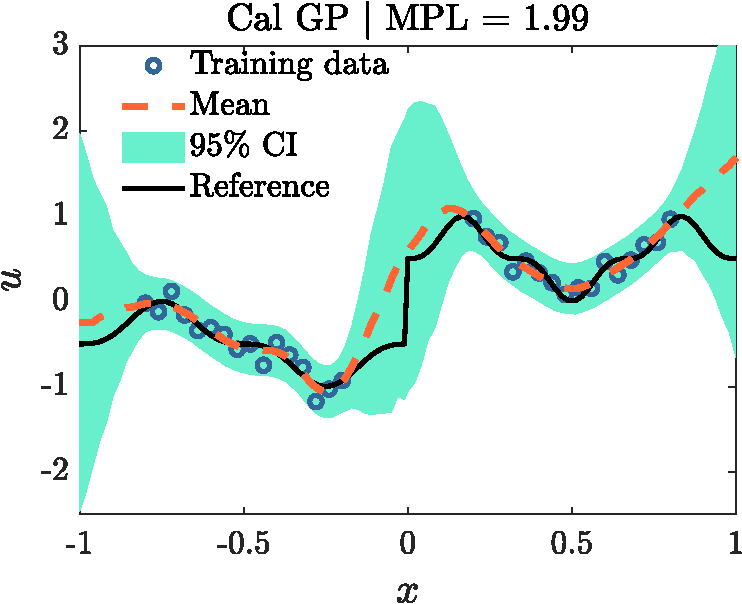
\includegraphics[width=0.32\textwidth]{./figs/fig1.pdf}}
		\subcaptionbox{}{}{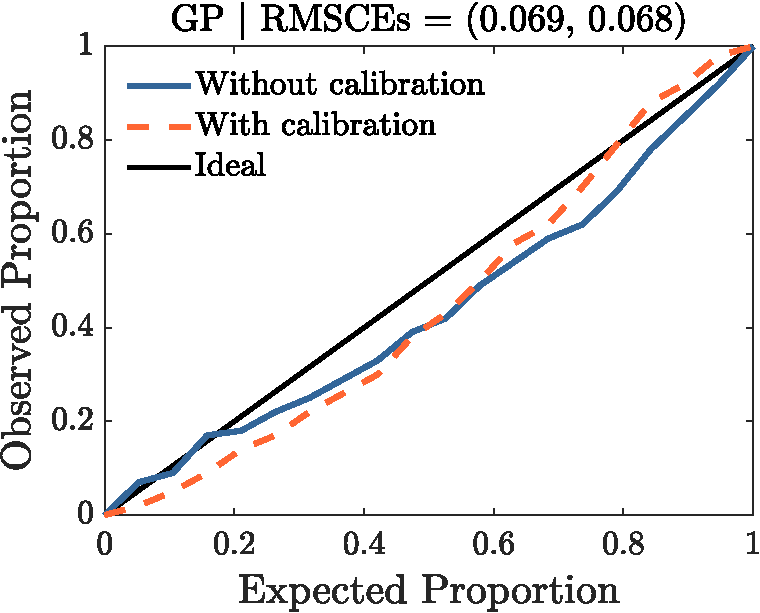
\includegraphics[width=0.32\textwidth]{./figs/fig2.pdf}}
		\caption{
			Caption.
		}
		\label{fig:label}
	\end{figure}

	\begin{table}[ht]
		\centering
		\footnotesize
		\begin{tabular}{c|c|c}
			\toprule
			\multicolumn{3}{c}{\textbf{Contents}}\\
			\midrule
			Problem & A & B\\
			\midrule
			Sections & A & B  \\
			\midrule
			\parbox[t]{2mm}{\multirow{5}{*}{\rotatebox[origin=c]{90}{Problem cases}}}& A & B  \\
			&  A & B \\
			& A & B \\
			\cline{2-3}
			& A & B  \\
			& A  & B  \\
			\bottomrule
		\end{tabular}
		\caption{
			Caption.
		}
		\label{tab:label}
	\end{table}
    
    \phantomsection 
    \addcontentsline{toc}{section}{Acknowledgment} 
    \section*{Acknowledgments}
    Acknowledgments.
    
    \phantomsection 
    \addcontentsline{toc}{section}{References} 
    \bibliographystyle{elsarticle-num-names}
    \bibliography{refs}
	
	\numberwithin{equation}{section}
	\numberwithin{figure}{section}
	\numberwithin{table}{section}
	\addtocontents{toc}{\protect\setcounter{tocdepth}{1}}
	
	\begin{appendices}
		
	\newpage
	\clearpage
	\section{Appendix title}\label{app:label}

\begingroup
\etocsetstyle {subsection}
{\leftskip 0pt}
{\leftskip 0pt}
{\bfseries\footnotesize\makebox[1cm][l]{\etocnumber}%
	\etocname\nobreak\hfill\nobreak\etocpage
	\par
	% \nointerlineskip
}
{}
\etocsetstyle {subsubsection}
{}
{\leftskip 30pt}
{\mdseries\footnotesize\makebox[1cm][l]{\etocnumber}%
	\etocname\nobreak\hfill\nobreak\etocpage
	\par
	% \nointerlineskip
}
{}
\localtableofcontentswithrelativedepth{+3}
\endgroup

\subsection{Appendix section title}
\label{app:label}

Text.


	
	\end{appendices}

\end{document}